\chapter[Les tableaux à 2 dimensions]{
Les tableaux à 2 dimensions}
\section{Définition}
{
La \textbf{dimension} d’un tableau est le nombre d’indices qu’on utilise
pour faire référence à un de ses éléments. À ne pas confondre avec la
taille !}

\begin{center}
 [Warning: Image ignored] % Unhandled or unsupported graphics:
%
\includegraphics[width=1.129cm,height=1.282cm]{log1-img/log1-img117}

\end{center}
{
Dans ce qui précède, nous avons introduit les tableaux à une dimension.
Un seul indice suffisait à localiser un de ses éléments. De nombreuses
situations nécessitent cependant l’usage de tableaux à deux dimensions.
Ils vous sont déjà familiers par leur présence dans beaucoup de
situations courantes : calendrier, grille horaire, grille de mots
croisés, sudoku, jeux se déroulant sur un quadrillage (damier,
échiquier, scrabble, …).}

\section{Déclaration}
{
Pour déclarer un tableau statique à 2 dimensions, on écrira :}

\begin{center}
 [Warning: Image ignored] % Unhandled or unsupported graphics:
%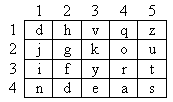
\includegraphics[width=1.129cm,height=1.282cm]{log1-img/log1-img118}

\end{center}
{\sffamily
nomTableau : \textbf{tableau} [ ligMin à ligMax, colMin à colMax] de
TypeElément}

{
Pour un tableau dynamique, on procédera en deux étapes comme expliqué
pour les tableaux à une dimension. On ne se permettra pas en logique de
combiner les deux types de tableaux, à savoir utiliser la notation
«~statique~» pour certaines dimensions et «~dynamique~» pour les
autres.}

{
Notez qu'un tableau à deux dimensions peut aussi être
vu comme un tableau à une dimension dont chacun des éléments est
lui-même un tableau à une dimension.}

{
\textbf{Exemple}\textbf{ : }Soit le tableau déclaré ainsi:}

{\sffamily
tabLettres : \textbf{tableau }[1 à 4, 1 à 5] de caractères}

{
On peut le visualiser à l’aide d’une grille à 4 lignes et 5 colonnes.}

{\centering   [Warning: Image ignored]
% Unhandled or unsupported graphics:
%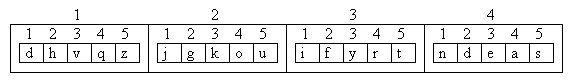
\includegraphics[width=4.577cm,height=2.699cm]{log1-img/log1-img119}
 \par}

{
Ainsi, la valeur de \textstyleCodeInsr{tabLettres[3,4]} est le caractère
‘r’. La vision «~tableau de tableau~» (ou décomposition en niveaux)
donnerait :}

  [Warning: Image ignored] % Unhandled or unsupported graphics:
%
\includegraphics[width=15.187cm,height=2.223cm]{log1-img/log1-img120}
 

{
Dans cette représentation, le tableau \textstyleCodeInsr{tabLettres} est
d’abord décomposé à un premier niveau en quatre éléments auxquels on
accède par le premier indice. Ensuite, chaque élément de premier niveau
est décomposé en cinq éléments de deuxième niveau accessibles par le
deuxième indice.}

\section{La troisième dimension (et au-delà)}
{
Certaines situations complexes nécessitent l'usage de
tableaux à 3 voire plus de dimensions.}

{
Pour déclarer un tableau statique à k dimensions, on écrira :}

{\sffamily
nomTableau : \textbf{tableau} [ bMin\_1 à bMax\_1, …, bMin\_k à bMax\_k]
de TypeElément}

\begin{center}
 [Warning: Image ignored] % Unhandled or unsupported graphics:
%
\includegraphics[width=1.129cm,height=1.282cm]{log1-img/log1-img121}

\end{center}
{
où chaque paire de bornes \textstyleCodeInsr{bMin\_i}~et
\textstyleCodeInsr{bMax\_i} limite l’indice correspondant à la ième
dimension du tableau.}

\section[Exercices]{ Exercices}
\liststyleExercice
\begin{enumerate}
\item {\sffamily\bfseries
Affichage}

{
Écrire un module qui affiche tous les éléments d'un
tableau à n lignes et m colonnes}
\end{enumerate}
\begin{enumerate}
\item {
ligne par ligne ;}
\item {
colonne par colonne.}
\end{enumerate}
\liststyleExercice
\begin{enumerate}
\item {\sffamily\bfseries
Les nuls}

{
Écrire un module qui reçoit un tableau (n x m)
d'entiers et qui affiche la proportion
d'éléments nuls dans ce tableau.}
\begin{center}
 [Warning: Image ignored] % Unhandled or unsupported graphics:
%
\includegraphics[width=1.134cm,height=1.134cm]{log1-img/log1-img122}

\end{center}
\item {\sffamily\bfseries
Le contour du tableau}
\end{enumerate}
{
On donne un tableau d’entiers tabEnt à n lignes et m colonnes. Écrire
\ un module retournant la somme de tous les éléments \textit{impairs}
situés sur le bord du tableau.}

\begin{center}
 [Warning: Image ignored] % Unhandled or unsupported graphics:
%\includegraphics[width=1.134cm,height=1.134cm]{log1-img/log1-img123}

\end{center}
{
Exemple : pour le tableau suivant, le module doit renvoyer 32}

\begin{center}
\tablehead{}
\begin{supertabular}{|m{0.62200004cm}|m{0.624cm}|m{0.624cm}|m{0.64100003cm}|}
\hline
\raggedleft  3 &
\raggedleft  4 &
\raggedleft  6 &
\raggedleft\arraybslash  11\\\hline
\raggedleft  2 &
\raggedleft  21 &
\raggedleft  7 &
\raggedleft\arraybslash  9\\\hline
\raggedleft  1 &
\raggedleft  5 &
\raggedleft  12 &
\raggedleft\arraybslash  3\\\hline
\end{supertabular}
\end{center}
{
Et pour le suivant, le module doit renvoyer 6}

\begin{center}
\tablehead{}
\begin{supertabular}{|m{0.27999997cm}|m{0.27999997cm}|m{0.27999997cm}|m{0.27999997cm}|m{0.297cm}|}
\hline
 4 &
 1 &
 2 &
 8 &
 5\\\hline
\end{supertabular}
\end{center}

\bigskip

\liststyleExercice
\setcounter{saveenum}{\value{enumi}}
\begin{enumerate}
\setcounter{enumi}{\value{saveenum}}
\item {\sffamily\bfseries
À vos pinceaux ! \ }
\end{enumerate}
{
On possède un tableau à n lignes et n colonnes dont les éléments de type
Couleur valent NOIR ou BLANC. On suppose que le tableau est initialisé
à ‘BLANC’ au départ. Écrire un module qui ‘noircit’ les cases de ce
tableau comme le suggèrent les dessins suivants~(les exemples sont
donnés pour un tableau 10 \textstylePolicepardfauti{x
}\textstylePolicepardfauti{10 mais les algorithmes doivent fonctionner
quelle que soit la taille du tableau).}}

{\centering   [Warning: Image ignored]
% Unhandled or unsupported graphics:
%
\includegraphics[width=11.499cm,height=3.313cm]{log1-img/log1-img124}
 \par}

\liststyleExercice
\setcounter{saveenum}{\value{enumi}}
\begin{enumerate}
\setcounter{enumi}{\value{saveenum}}
\item {\sffamily\bfseries
Le tableau de cotes}

{
Soit un tableau à n lignes et m colonnes d'entiers où
une ligne représente les notes sur 20 d'un étudiant et
les colonnes toutes les notes d'un cours.}

{
Écrire un algorithme recevant ce tableau en paramètre et affichant le
pourcentage d'étudiants ayant obtenu une moyenne
supérieure à 50\%.}
\item {\sffamily\bfseries
Tous positifs}
\end{enumerate}
{
Écrire un module qui reçoit un tableau (n x m) d’entiers et qui vérifie
si tous les nombres qu’il contient sont strictement positifs. Bien sûr,
on veillera à éviter tout travail inutile; la rencontre d’un nombre
négatif doit arrêter le module.}

\begin{center}
 [Warning: Image ignored] % Unhandled or unsupported graphics:
%
\includegraphics[width=1.134cm,height=1.134cm]{log1-img/log1-img125}

\end{center}
\liststyleExercice
\setcounter{saveenum}{\value{enumi}}
\begin{enumerate}
\setcounter{enumi}{\value{saveenum}}
\item {\sffamily\bfseries
Le carré magique}
\end{enumerate}
{
Un carré magique est un tableau d’entiers carré
(c'est-à-dire possédant autant de lignes que de
colonnes) ayant la propriété suivante: si on additionne les éléments
d'une quelconque de ses lignes, de ses colonnes ou de
ses deux diagonales, on obtient à chaque fois le même résultat.}

\begin{center}
 [Warning: Image ignored] % Unhandled or unsupported graphics:
%\includegraphics[width=1.134cm,height=1.134cm]{log1-img/log1-img126}

\end{center}
{
Écrire un module recevant en paramètres le tableau[1 à n, 1 à n]
d'entiers Carré et renvoyant une valeur booléenne
indiquant si Carré est un carré magique ou non.}

\liststyleExercice
\setcounter{saveenum}{\value{enumi}}
\begin{enumerate}
\setcounter{enumi}{\value{saveenum}}
\item[] 
\bigskip
\item {\sffamily\bfseries
Le contour du tableau}
\end{enumerate}
{
On donne un tableau d’entiers tabEnt à n lignes et m colonnes. Écrire
\ un module retournant la somme de tous les éléments \textit{impairs}
situés sur le bord du tableau.}

\begin{center}
 [Warning: Image ignored] % Unhandled or unsupported graphics:
%\includegraphics[width=1.134cm,height=1.134cm]{log1-img/log1-img127}

\end{center}
{
Exemple : pour le tableau suivant, le module doit renvoyer 32}

\begin{center}
\tablehead{}
\begin{supertabular}{|m{0.62200004cm}|m{0.624cm}|m{0.624cm}|m{0.64100003cm}|}
\hline
\raggedleft  3 &
\raggedleft  4 &
\raggedleft  6 &
\raggedleft\arraybslash  11\\\hline
\raggedleft  2 &
\raggedleft  21 &
\raggedleft  7 &
\raggedleft\arraybslash  9\\\hline
\raggedleft  1 &
\raggedleft  5 &
\raggedleft  12 &
\raggedleft\arraybslash  3\\\hline
\end{supertabular}
\end{center}
{
Et pour le suivant, le module doit renvoyer 6}

\begin{center}
\tablehead{}
\begin{supertabular}{|m{0.27999997cm}|m{0.27999997cm}|m{0.27999997cm}|m{0.27999997cm}|m{0.297cm}|}
\hline
 4 &
 1 &
 2 &
 8 &
 5\\\hline
\end{supertabular}
\end{center}

\bigskip

\liststyleExercice
\setcounter{saveenum}{\value{enumi}}
\begin{enumerate}
\setcounter{enumi}{\value{saveenum}}
\item {\sffamily\bfseries
À vos pinceaux ! \ }
\end{enumerate}
{
On possède un tableau à n lignes et n colonnes dont les éléments de type
Couleur valent NOIR ou BLANC. On suppose que le tableau est initialisé
à ‘BLANC’ au départ. Écrire un module qui ‘noircit’ les cases de ce
tableau comme le suggèrent les dessins suivants~(les exemples sont
donnés pour un tableau 10 \textstylePolicepardfauti{x
}\textstylePolicepardfauti{10 mais les algorithmes doivent fonctionner
quelle que soit la taille du tableau).}}

{\centering   [Warning: Image ignored]
% Unhandled or unsupported graphics:
%
\includegraphics[width=11.499cm,height=3.313cm]{log1-img/log1-img128}
 \par}

\liststyleExercice
\setcounter{saveenum}{\value{enumi}}
\begin{enumerate}
\setcounter{enumi}{\value{saveenum}}
\item {\sffamily\bfseries
Le triangle de Pascal}
\end{enumerate}
{
Le triangle de Pascal est construit de la façon suivante : }

\liststyleListi
\begin{itemize}
\item {
la ligne initiale contient un seul élément de valeur 1 ;}
\item {
chaque ligne possède un élément de plus que la précédente ;}
\item {
chaque ligne commence et se termine par 1 ;}
\item {
pour calculer un nombre d’une autre case du tableau, on additionne le
nombre situé dans la case située juste au-dessus avec celui dans la
case à la gauche de la précédente. }
\end{itemize}
{
Écrire un module qui reçoit en paramètre un entier
\textstyleCodeInsr{n}, et qui renvoie un tableau \ contenant les
\textstyleCodeInsr{n+1} premières lignes du triangle de Pascal
(indicées de \textstyleCodeInsr{0} à \textstyleCodeInsr{n}).
N.B.: le «~triangle~» sera bien entendu renvoyé dans un tableau carré.
Quid des cases \ non occupées ?}

{
Par exemple, pour n = 5, on aura le tableau suivant :}

\begin{center}
\begin{minipage}{3.191cm}
\begin{center}
\tablehead{}
\begin{supertabular}{|m{0.33600003cm}|m{0.33600003cm}|m{0.33600003cm}|m{0.33600003cm}|m{0.33600003cm}|m{0.31200004cm}|}
\hline
 1 &
~
 &
~
 &
~
 &
~
 &
~
\\\hline
 1 &
 1 &
~
 &
~
 &
~
 &
~
\\\hline
 1 &
 2 &
 1 &
~
 &
~
 &
~
\\\hline
 1 &
 3 &
 3 &
 1 &
~
 &
~
\\\hline
 1 &
 4 &
 6 &
 4 &
 1 &
~
\\\hline
 1 &
 5 &
 10 &
 10 &
 5 &
 1\\\hline
\end{supertabular}
\end{center}

\bigskip
\end{minipage}
\end{center}

\bigskip


\bigskip


\bigskip

\liststyleExercice
\begin{enumerate}
\item {\sffamily\bfseries
Le calendrier du mois}
\end{enumerate}
{
Écrire \ un module qui reçoit en paramètres le numéro du premier jour du
mois 
(c-à-d 1 si le mois commence un lundi, 2 si le mois commence un mardi,
etc.) ainsi que le nombre de jours dans le mois. Au départ de ces
données, le module remplira avec les dates des jours du mois un tableau
«~calendrier~» à deux dimensions, dont les colonnes représentent les
jours (la première colonne correspondant au lundi) et les lignes les
semaines. Par exemple, si le mois contient 30 jours et le premier jour
est un mercredi, le contenu du tableau sera :}

\begin{center}
\tablehead{}
\begin{supertabular}{|m{0.807cm}|m{0.807cm}|m{0.807cm}|m{0.807cm}|m{0.807cm}|m{0.807cm}|m{0.81100005cm}|}
\multicolumn{1}{m{0.807cm}}{\centering 
\textstylePolicepardfauti{L}} &
\multicolumn{1}{m{0.807cm}}{\centering 
\textstylePolicepardfauti{M}} &
\multicolumn{1}{m{0.807cm}}{\centering 
\textstylePolicepardfauti{M}} &
\multicolumn{1}{m{0.807cm}}{\centering 
\textstylePolicepardfauti{{J}}} &
\multicolumn{1}{m{0.807cm}}{\centering 
\textstylePolicepardfauti{{V}}} &
\multicolumn{1}{m{0.807cm}}{\centering 
\textstylePolicepardfauti{{S}}} &
\multicolumn{1}{m{0.81100005cm}}{\centering\arraybslash
 \textstylePolicepardfauti{D}}\\\hline
~
 &
~
 &
\raggedleft  \textstylePolicepardfauti{1} &
\raggedleft  \textstylePolicepardfauti{2} &
\raggedleft  \textstylePolicepardfauti{3} &
\raggedleft  \textstylePolicepardfauti{4} &
\raggedleft\arraybslash 
\textstylePolicepardfauti{5}\\\hline
\raggedleft  \textstylePolicepardfauti{6} &
\raggedleft  \textstylePolicepardfauti{7} &
\raggedleft  \textstylePolicepardfauti{8} &
\raggedleft  \textstylePolicepardfauti{9} &
\raggedleft  \textstylePolicepardfauti{10} &
\raggedleft  \textstylePolicepardfauti{11} &
\raggedleft\arraybslash 
\textstylePolicepardfauti{12}\\\hline
\raggedleft  \textstylePolicepardfauti{13} &
\raggedleft  \textstylePolicepardfauti{14} &
\raggedleft  \textstylePolicepardfauti{15} &
\raggedleft  \textstylePolicepardfauti{16} &
\raggedleft  \textstylePolicepardfauti{17} &
\raggedleft  \textstylePolicepardfauti{18} &
\raggedleft\arraybslash 
\textstylePolicepardfauti{19}\\\hline
\raggedleft  \textstylePolicepardfauti{20} &
\raggedleft  \textstylePolicepardfauti{21} &
\raggedleft  \textstylePolicepardfauti{22} &
\raggedleft  \textstylePolicepardfauti{23} &
\raggedleft  \textstylePolicepardfauti{24} &
\raggedleft  \textstylePolicepardfauti{25} &
\raggedleft\arraybslash 
\textstylePolicepardfauti{26}\\\hline
\raggedleft  \textstylePolicepardfauti{27} &
\raggedleft  \textstylePolicepardfauti{28} &
\raggedleft  \textstylePolicepardfauti{29} &
\raggedleft  \textstylePolicepardfauti{30} &
~
 &
~
 &
~
\\\hline
\end{supertabular}
\end{center}
{
Réflexions~: }

\liststyleListi
\begin{itemize}
\item {
Combien de lignes au maximum doit avoir ce tableau ?}
\item {
Quid des cases non occupées ?}
\end{itemize}

\bigskip

\liststyleExercice
\begin{enumerate}
\item {\sffamily\bfseries
À vos pinceaux \ (la suite) ! \ }
\end{enumerate}
{
Pour poursuivre l'exercice du pinceau, voici quelques
cas plus coriaces\textstylePolicepardfauti{.}}

{\centering \par}

\begin{center}
 [Warning: Image ignored] % Unhandled or unsupported graphics:
%
\includegraphics[width=11.94cm,height=3.438cm]{log1-img/log1-img129}

\end{center}
\liststyleExercice
\setcounter{saveenum}{\value{enumi}}
\begin{enumerate}
\setcounter{enumi}{\value{saveenum}}
\item {\sffamily\bfseries
Exercices sur la complexité}
\end{enumerate}
\liststyleNumberingv
\begin{enumerate}
\item {
Quelle est la complexité d’un algorithme de parcours
d'un tableau n x n ?}
\item {
\textstylePolicepardfauti{Et pour un algorithme qui remet à 0 toutes les
occurrences du maximum d'un tableau \ n x n ?}}
\item {
\textstylePolicepardfauti{Quelle est la complexité de
l'algorithme que vous avez écrit pour résoudre les
exercices du pinceau ?}}
\end{enumerate}
\liststyleExercice
\begin{enumerate}
\item {\sffamily\bfseries
Lignes et colonnes}
\end{enumerate}
{
\textstylePolicepardfauti{\textcolor{black}{Écrire un module qui reçoit
un tableau d’entiers à 2 dimensions en paramètre et qui retourne un
booléen indiquant si ce tableau possède 2 lignes ou 2 colonnes
identiques. }}}

{
\textstylePolicepardfauti{\textcolor{black}{Dans l’affirmative, ce
module renverra également en paramètres les informations suivantes :}}}

\begin{itemize}
\item {\color{black}
les indices des lignes ou colonnes identiques}
\item {\color{black}
un caractère valant ‘L’ ou ‘C’ selon qu’il s’agit de lignes ou de
colonnes}
\end{itemize}
{\color{black}
Dans la négative, les valeurs de ces paramètres seront indéterminées ou
quelconques, elles ne seront de toute façon pas utilisées par le module
appelant.}


\bigskip

